\documentclass{beamer}
\usepackage{amsfonts,amsmath,oldgerm}

\usepackage[utf8]{inputenc}
\usepackage[T1]{fontenc}
\usepackage{graphicx}
\usepackage{listings}
\usepackage{hyperref}
\usepackage{verbatim}
\usepackage{siunitx}

\usepackage[english]{babel}
\usepackage[export]{adjustbox}
\usepackage{caption} %For subfigures
\usepackage{subcaption} %For subfigures
\usepackage{placeins} %FloatBarriers

\usetheme{sintef}

\newcommand{\testcolor}[1]{\colorbox{#1}{\textcolor{#1}{test}}~\texttt{#1}}

\usefonttheme[onlymath]{serif}
\graphicspath{{assets/images/}}


\titlebackground*{assets/logos/background}

\newcommand{\hrefcol}[2]{\textcolor{cyan}{\href{#1}{#2}}}

\title{Numerical study of the airflow over a high-altitude pseudo-satellite wing}
\subtitle{PhD update}

\author{\href{mailto:mail@carlobrunelli.com}{Carlo Brunelli}}


\newcommand{\VV}[1] {\vv{\vv{#1}}}

\begin{document}
\maketitle


\begin{frame}

PhD presentation after 1.5 years

\end{frame}

\section{Numerical Methods}
\begin{frame}{Numerical Method implemented}
The numerical method currently implemented are:
  \begin{itemize}
    \item Variational Multiscale Method (VMS)
    \item Streamline upwind Petrov–Galerkin (SUPG)
  \end{itemize} 

Different solution method are available for all of them 
  \begin{itemize}
    \item Non-linear (NLIN)
    \item Linearized-Coupled (LC-VMS)
    \item Linearized-Segregated (LS-VMS)
  \end{itemize} 
\end{frame}


\begin{frame}{Variational Multiscale Method}
  \begin{itemize}
    \item Evolution of the SUPG
    \item Implict LES
    \item It does not need calibration
    \item Residual-based stabilization
  \end{itemize} 
\end{frame}


\begin{frame}{Galkerkin formulation}
Conservation of mass:
\begin{equation}
    \nabla\cdot \Vec{u} = 0
    \label{equfo:cont}
\end{equation}

Conservation of momentum:
\begin{equation}
    \dfrac{\partial \Vec{u}}{\partial t} + (\Vec{u}\cdot\nabla)\Vec{u} + \nabla p - \nu\Delta\Vec{u} - f = 0
        \label{equfo:mom}
\end{equation}

Variational Formulation
\begin{equation}
\begin{split}
  B^G = &   \int_\Omega \dfrac{\partial \Vec{u}}{\partial t}\cdot \Vec{v}\;d\Omega +
    \int_\Omega(\Vec{u}\cdot\nabla)\Vec{u}\cdot \Vec{v} \;d\Omega+ 
    \int_\Omega \nabla (p)\cdot\Vec{v} \;d\Omega + \\
     & + \int_\Omega\nu\nabla\Vec{u}\cdot\nabla\Vec{v} \;d\Omega  -
        \int_\Omega f\cdot\Vec{v} \;d\Omega + 
    \int_\Omega q(\nabla \cdot \Vec{u})\;d\Omega = 0
    \end{split}
    \label{equ:weak}
\end{equation}

\end{frame}

\begin{frame}{Stabilization equations}
\begin{equation}
B^{SUPG}(t, (\Vec{u},p), (\Vec{v},q))  =     \int_\Omega(\tau_m(\Vec{u}\cdot\nabla \Vec{v} +\nabla q)\cdot\Vec{R_m} \;d\Omega+ \int_\Omega \tau_c (\nabla \cdot \Vec{v})R_c \;d\Omega
\label{equ:bsupg}
\end{equation}

\begin{equation}
B^{VMS1}(t, (\Vec{u},p), (\Vec{v},q))  = \int_\Omega (\Vec{u}\cdot\nabla \Vec{v}')\odot(\tau_m \Vec{R_m}) \;d\Omega
\label{equ:bvms1}
\end{equation}


\begin{equation}
B^{VMS2}(t, (\Vec{u},p), (\Vec{v},q))  = -\int_\Omega (\nabla\Vec{v}\odot(\tau_m \Vec{R_m} \otimes \tau_m \Vec{R_m}) \;d\Omega
\label{equ:bvms2}
\end{equation}

\end{frame}


\begin{frame}{Stabilization parameters}

\begin{equation}
\tau_m =\bigg( \dfrac{4}{\Delta t^2} + \Vec{u}\cdot{G}\Vec{u} + C_I \nu^2 {G}:{G} \bigg)^{-1/2}
\label{equ:taum}
\end{equation}

\begin{equation}
\tau_c = (\tau_c\Vec{g}\cdot\Vec{g})^{-1}
\label{equ:tauc}
\end{equation}

Where G is the inverse of the gradient of the map cell.
For a cubed shaped element, with $h$ the edge length, $G_{ij} =\dfrac{1}{h^2}\delta_{ij}$, where $\delta_{ij}$ is the Kronecker delta.

\end{frame}


\begin{frame}{Linearization}
Using Taylor's expansion for velocity:
\begin{equation}
    \Vec{u}_{adv} = 2.1875 u^{n} - 2.1875 u^{n-1} + 1.3125 u^{n-2} - 0.3125 u^{n-3} 
    \label{equlin:taylor_exp}
\end{equation}

\begin{equation}
 (\Vec{u}\cdot\nabla)\Vec{u} \Rightarrow  (\Vec{u}_{adv}\cdot\nabla)\Vec{u} 
\end{equation}

$\Vec{u}_{adv}$ used also for computing stabilization parameters


\end{frame}

\begin{frame}{Linearization}
\begin{equation}
  \begin{split}
  B^G(t, (\Vec{u},p), (\Vec{v},q))  = &  \int_\Omega \dfrac{\partial \Vec{u}}{\partial t}\cdot \Vec{v}\;d\Omega +
      \int_\Omega(\Vec{u}_{adv}\cdot\nabla)\Vec{u}\cdot \Vec{v} \;d\Omega+ 
      \int_\Omega \nabla (p)\cdot\Vec{v} \;d\Omega + \\
      & + \int_\Omega\nu\nabla\Vec{u}\cdot\nabla\Vec{v} \;d\Omega  -
          \int_\Omega f\cdot\Vec{v} \;d\Omega + 
      \int_\Omega q(\nabla \cdot \Vec{u})\;d\Omega
  \end{split}
      \label{equ:Bglin}
  \end{equation}
  
  \begin{equation}
  B^{SUPG,lin}(t, (\Vec{u},p), (\Vec{v},q))  =     \int_\Omega(\tau_m(\Vec{u}_{adv}\cdot\nabla \Vec{v} +\nabla q)\cdot\Vec{R_{m,lin}} \;d\Omega+ \int_\Omega \tau_c (\nabla \cdot \Vec{v})R_c \;d\Omega
  \label{equ:bsupglin}
  \end{equation}
  
  \begin{equation}
  B^{VMS1,lin}(t, (\Vec{u},p), (\Vec{v},q))  = \int_\Omega (\Vec{u}_{adv}\cdot\nabla \Vec{v}')\odot(\tau_m \Vec{R_{m,lin}}) \;d\Omega
  \label{equ:bvms1lin}
  \end{equation}
\end{frame}


\begin{frame}{ODE Solver}
Employing $\theta$-method for time marching. $\theta=0.5$ for velocity and $\theta=1.0$ for pressure to avoid un-smoothed oscillations
\begin{figure}
  \centering
  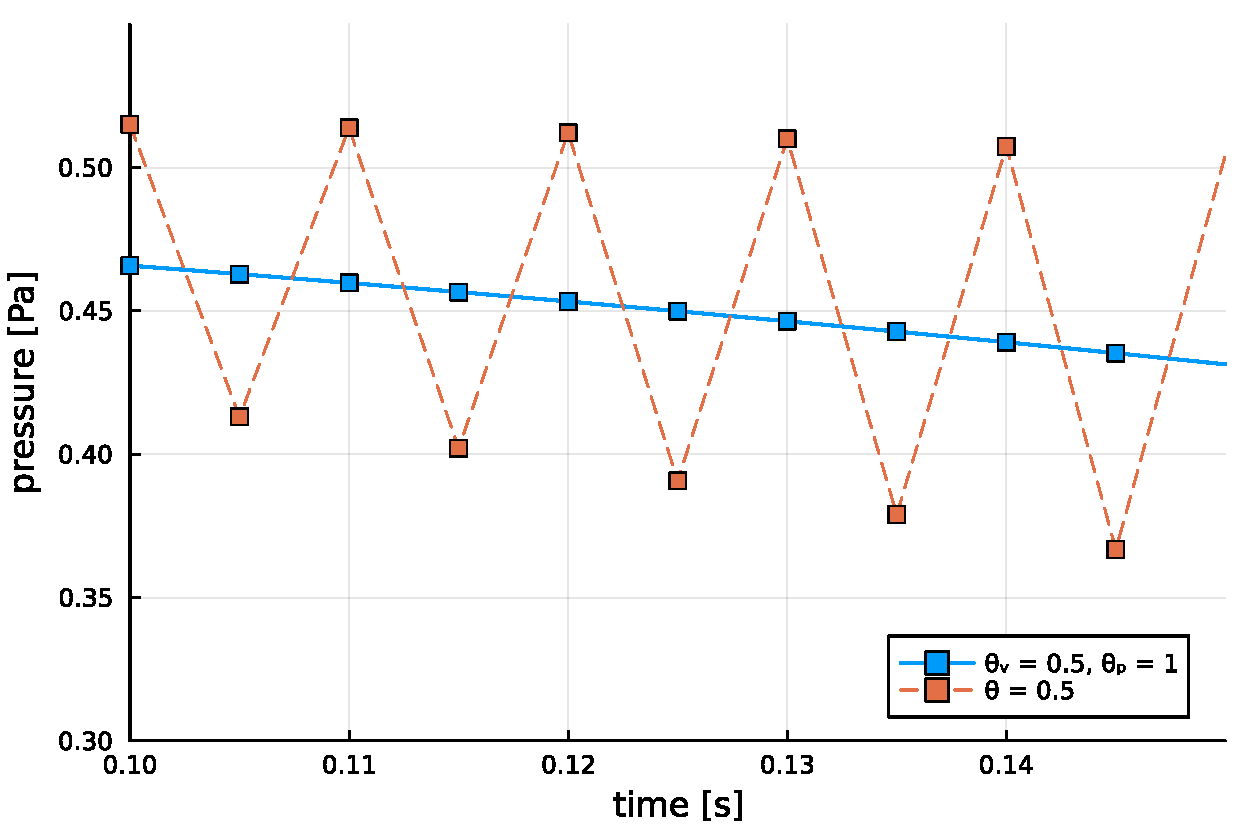
\includegraphics[width=0.45\textwidth]{Theta_stab_nstab.pdf}
  \caption{Pressure oscillations}
\end{figure} 
\end{frame}


\begin{frame}{Segregated formulation}
\begin{equation}
  T\dfrac{\partial \Vec{x}}{\partial t} + A \Vec{x} = 0
  \label{equseg:eq1}
\end{equation}
Applying the $\theta$-method

\begin{equation}
      T\dfrac{\partial \Vec{x}}{\partial t} = - A \Vec{x}
      \label{equseg:eq2}
\end{equation}


\begin{equation}
      T\dfrac{\Vec{x}^{n+1}-\Vec{x}^{n}}{\Delta t} = - \bigg ( A \Vec{x}^{n+1}\theta + A\Vec{x}^n(1-\theta) \bigg )
      \label{equseg:eq3}
\end{equation}

\begin{equation}
      \bigg (\dfrac{T}{\Delta t}+A\theta \bigg )(\Vec{x}^{n+1}-\Vec{x}^{n}) = - A \Vec{x}^{n}
\end{equation}
  
\end{frame}

\begin{frame}{Matrices splitting}

  Splitting the problem in solving velocity and pressure field:
\begin{equation}
  A = \begin{bmatrix}
A_{pp} & A_{pu}\\
A_{up} & A_{uu}
\end{bmatrix}
\end{equation}

\begin{equation}
  T = \begin{bmatrix}
  0 & T_{pu}\\
  0 & T_{uu}
\end{bmatrix}
\end{equation}


Thanks to the stabilization the matrix $A_{pp}$ is nonzero. This translates into nonzero diagonal elements, reducing the conditioning number of the matrix and improving the overall stability of the method.

\end{frame}


\begin{frame}
Introducing the time step increments and the acceleration terms:
$$\Delta u = u^{n+1}-u^{n}$$
$$\Delta p = p^{n+1}-p^{n}$$
$$a = \Delta u / \Delta t$$

The linear system will be solved in an iterative manner. Two following iterations are marked as $m$ and $m+1$, and the difference between two following iteration is:
$$\Delta a = a^{m+1}-a^m$$
$$\Delta p^{m+1} = a^{m+1}-a^m$$
$$u^m=u^n+\Delta t a^m$$
$$p^m = p^n + \sum_{i=0}^m \Delta p^i$$
\end{frame}

\begin{frame}
  \begin{equation}
    \begin{split}
    (T_{uu}+\theta \Delta t A_{uu})\bm{\Delta a^*} = -A_{uu}u^m- Au_{up}p^m - (T_{uu}+\theta\Delta t A_{uu})a^m+A_{uu}\Delta t a^m +\\+ A_{uu}\Delta t a^m + (1-\theta)A_{up}\sum_{i=0}^m \Delta p^i  
  \end{split}
  \label{equseg:mom1}
\end{equation}

\begin{equation}
  \begin{split}
  \bigg( (T_{pu}+\Delta t A_{pu})(T_{uu}+\theta\Delta t A_{uu})^{-1} \theta A_{up} - App \bigg ) \bm{\Delta p^{m+1}} = \\= T_{pu}\Delta a^* + A_{pu}(u^m+\Delta t\Delta a^*)+A_{pp}p^m+T_{pu}a^m
\end{split}
\label{equseg:cont1}
\end{equation}
\end{frame}

\begin{frame}
  It is possible to apply a multicorrector-predictor iterative scheme. At the beginning of each time step the velocity, pressure, and acceleration are initialized as:
\begin{itemize}
\item $u^0 = u^n$
\item $p^0 = p^n$
\item $a^0 = 0$
\item $\sum_{i=0}^m \Delta p^i = 0$
\end{itemize}

Then the iterative process begins:

\begin{enumerate}
    \item Solve linear system \eqref{equseg:mom1} for $\Delta a^*$
    \item Solve linear system \eqref{equseg:cont1} for $\Delta p^{m+1}$
    \item Compute $\Delta a = \Delta a^* - (T_{uu}+\theta\Delta t A_{uu})^{-1}\theta A_{up}  \Delta p^{m+1}$
    \item Update $a^{m+1} = a^m + \Delta a$
    \item Update $u^{m+1} = u^m + \Delta a \Delta t$
    \item Update $p^{m+1} = p^m +\Delta p^{m+1}$
\end{enumerate}

\end{frame}


\section{Performances}
\begin{frame}{Weak Scaling}
Weak scalability: the solution time almost does not change with constant problem size per processor
\begin{figure}
         \centering
         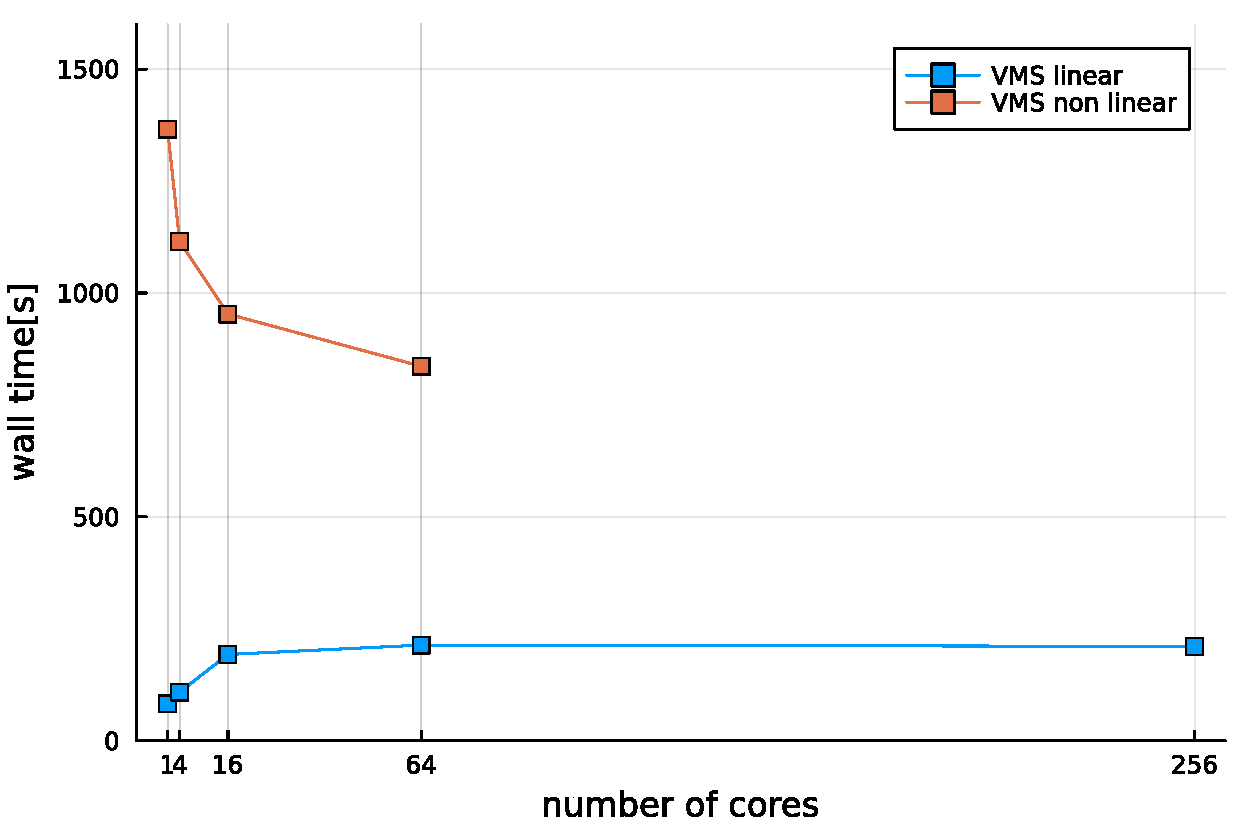
\includegraphics[width=0.5\textwidth]{TaylorGreen_Weak_Scalability_VMS_lin_nlin.pdf}
         \caption{Taylor Green weak scalability}
\end{figure} 
\end{frame}

\begin{frame}{Strong Scaling}
Strong scalability: doubling the number of processors halves the solution time

\begin{figure}
         \centering
         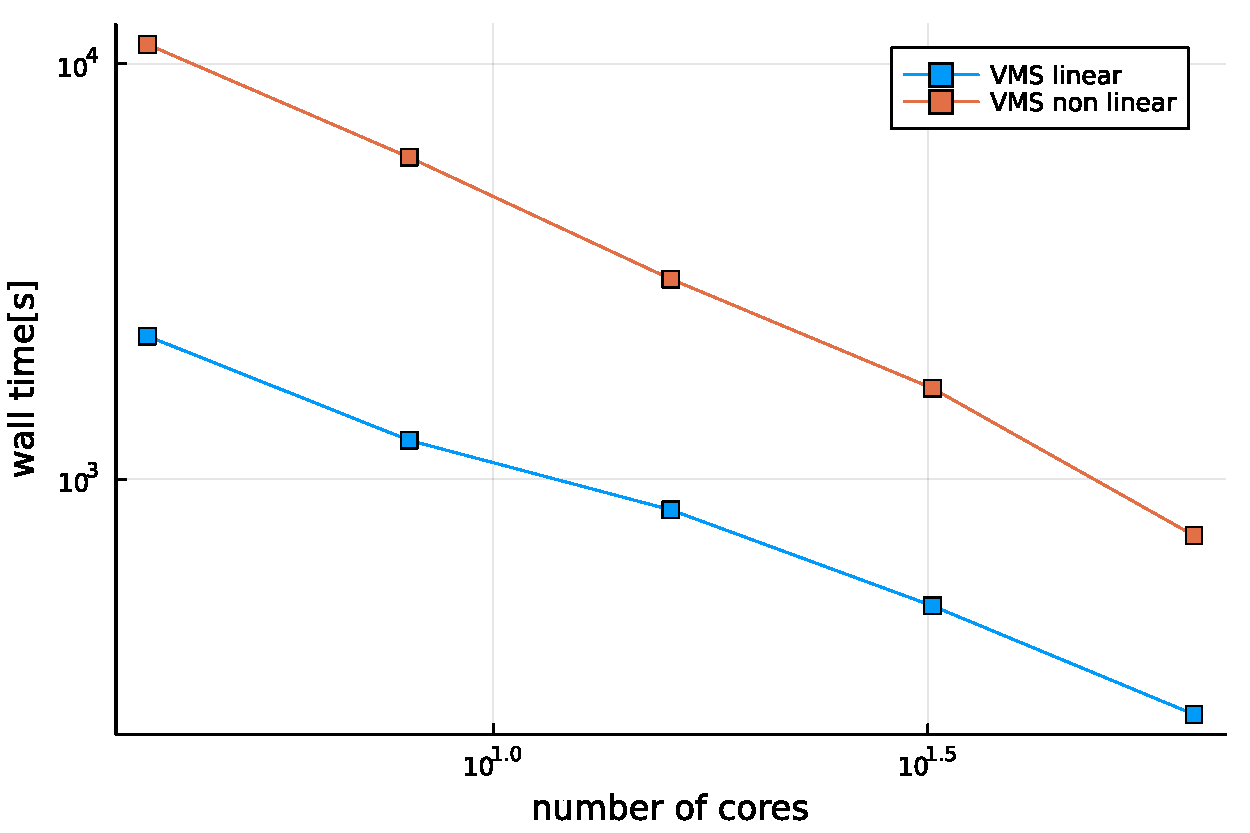
\includegraphics[width=0.5\textwidth]{TaylorGreen_Strong_Scalability_VMS_lin_nlin.pdf}
         \caption{Taylor Green Strong scalability}
\end{figure} 
\end{frame}

\section{Synthetic Eddy Method}
\begin{frame}{SyntheticEddyMethod.jl}
\begin{itemize}
\item \href{https://www.theoj.org/joss-papers/joss.05565/10.21105.joss.05565.pdf}{publication}
\item presented at \textit{JuliaCon2023} at MIT
\end{itemize}

Features:
\begin{itemize}
\item Create fluctuations that respect the divergence-free condition (DFSEM)
\item Create velocity fluctuations for inlet boundary conditions
\item Create coherent eddies in 3D domain
\item Define custom Reynolds Stress Tensor
\item Import from file custom Reynolds Stress Tensor
\end{itemize}
\end{frame}


\begin{frame}{Synthetic Eddy Method}
Reynolds decomposition:
\begin{equation}
    \Vec{u}(\Vec{x},t) = \Vec{U}(\Vec{x},t) +  \Vec{u'}(\Vec{x},t)
    \label{sem:u}
\end{equation}

Compute velocity fluctuations, using a suitable shape function:
\begin{equation}
u_i(\boldsymbol{x})=U_i(\boldsymbol{x})+\frac{1}{\sqrt{N}} \sum_{k=1}^N a_{i j} \epsilon_j^k f_{\sigma(\boldsymbol{x})}\left(\boldsymbol{x}-\boldsymbol{x}^k\right)
\label{sem:ui}
\end{equation}
\end{frame}


\section{Laminar Separation Bubble}




\begin{frame}{Simulations}
\begin{itemize}
\item VMS linearized coupled sd7003s - Re $\num{60000}$ - AoA $\ang{4}$ 
\item VMS linearized segregated DU89 - Re $\num{250000}-\num{500000}$ - AoA $\ang{1}-\ang{5}$ 
\end{itemize}
\end{frame}

\begin{frame}{Models}
sd7003s - Re $\num{60000}$ - AoA $\ang{4}$ 
\begin{figure}[h]
     \centering          
         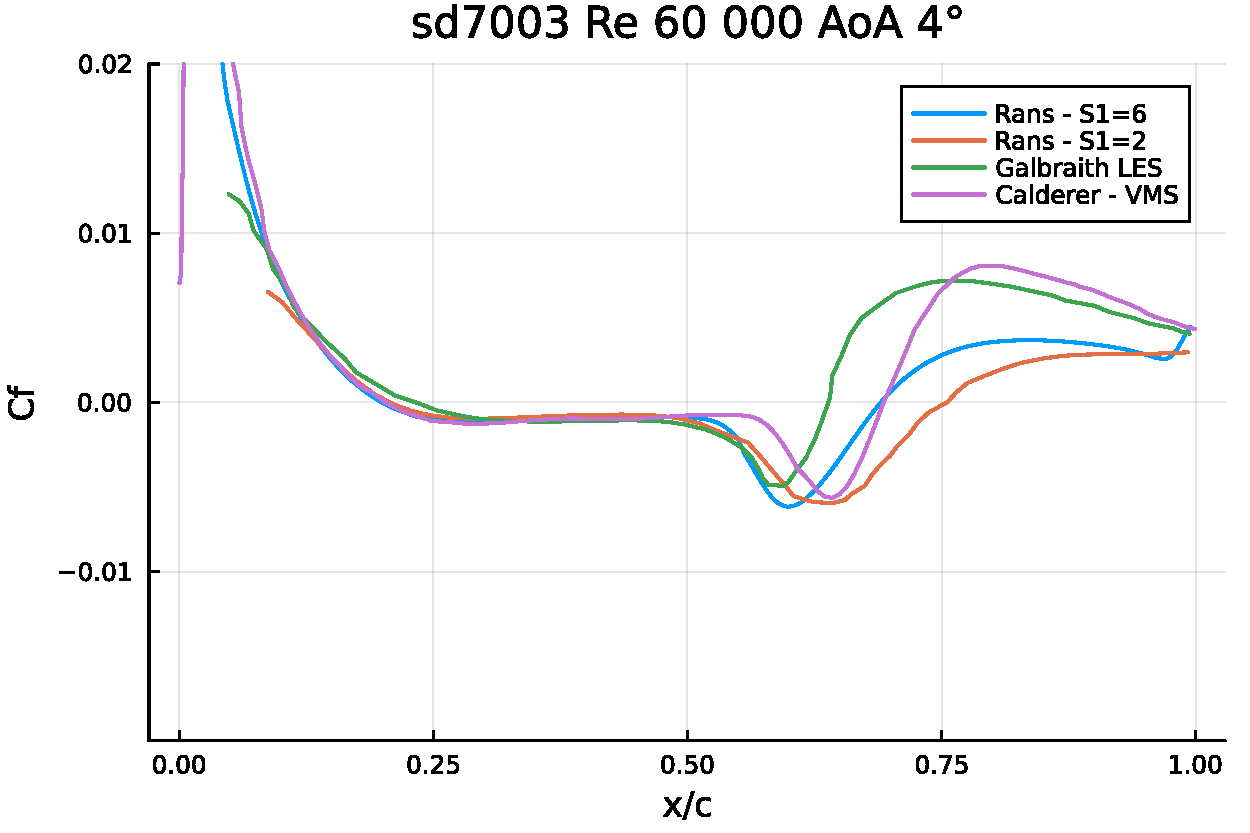
\includegraphics[width=0.65\textwidth]{ sd7003_differentmodels.pdf}
         \caption{Different model provides different results. RANs use $\gamma -Re_ \theta$ model.}
     \end{figure} 
\end{frame}

\begin{frame}{VMS linearized coupled sd7003s}
Copuled: velocity and pressure are solved at the same time.
Re $\num{60000}$ - AoA $\ang{4}$ . Initialization with velocity-ramping
\begin{figure}[h]
     \centering          
     \begin{subfigure}[h]{0.45\textwidth}
              \centering
         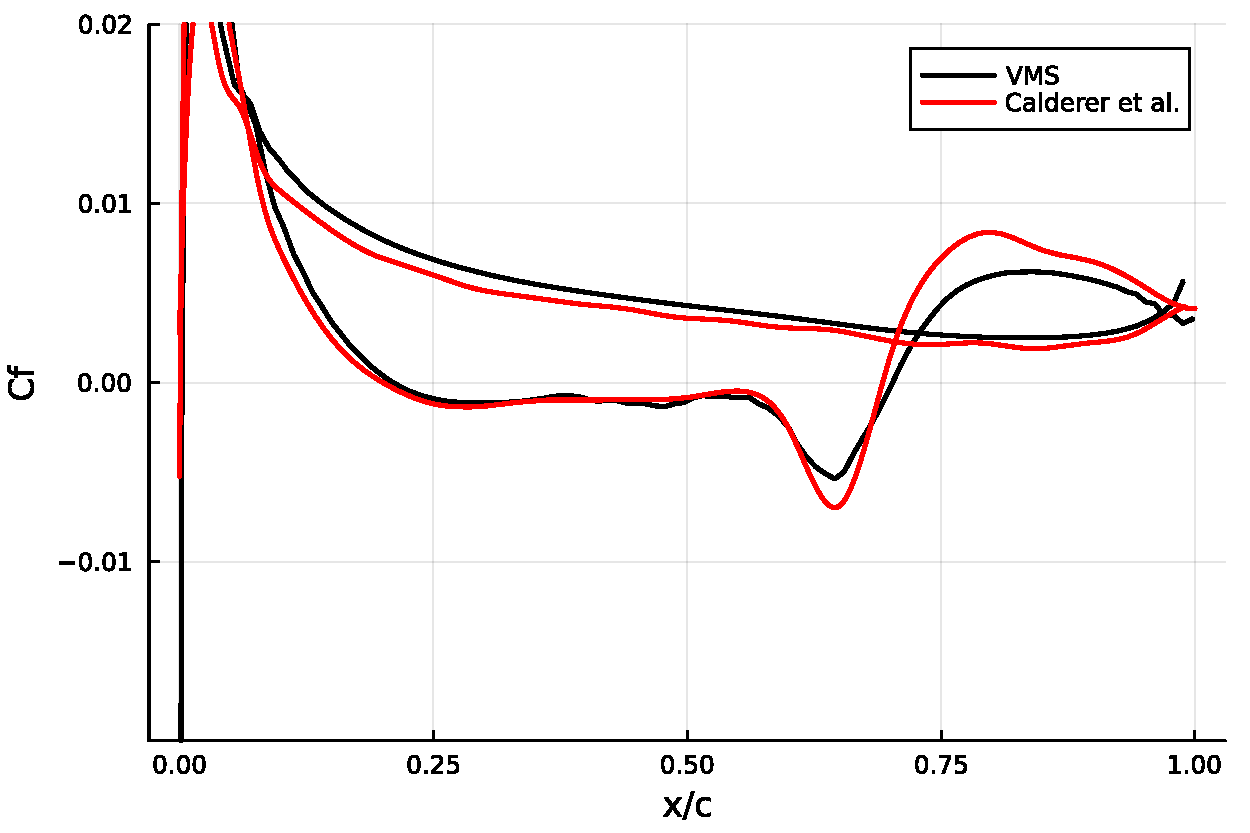
\includegraphics[width=\textwidth]{sd7003_cf.pdf}
    \end{subfigure}
          \hfill
     \begin{subfigure}[h]{0.45\textwidth}
      \centering
         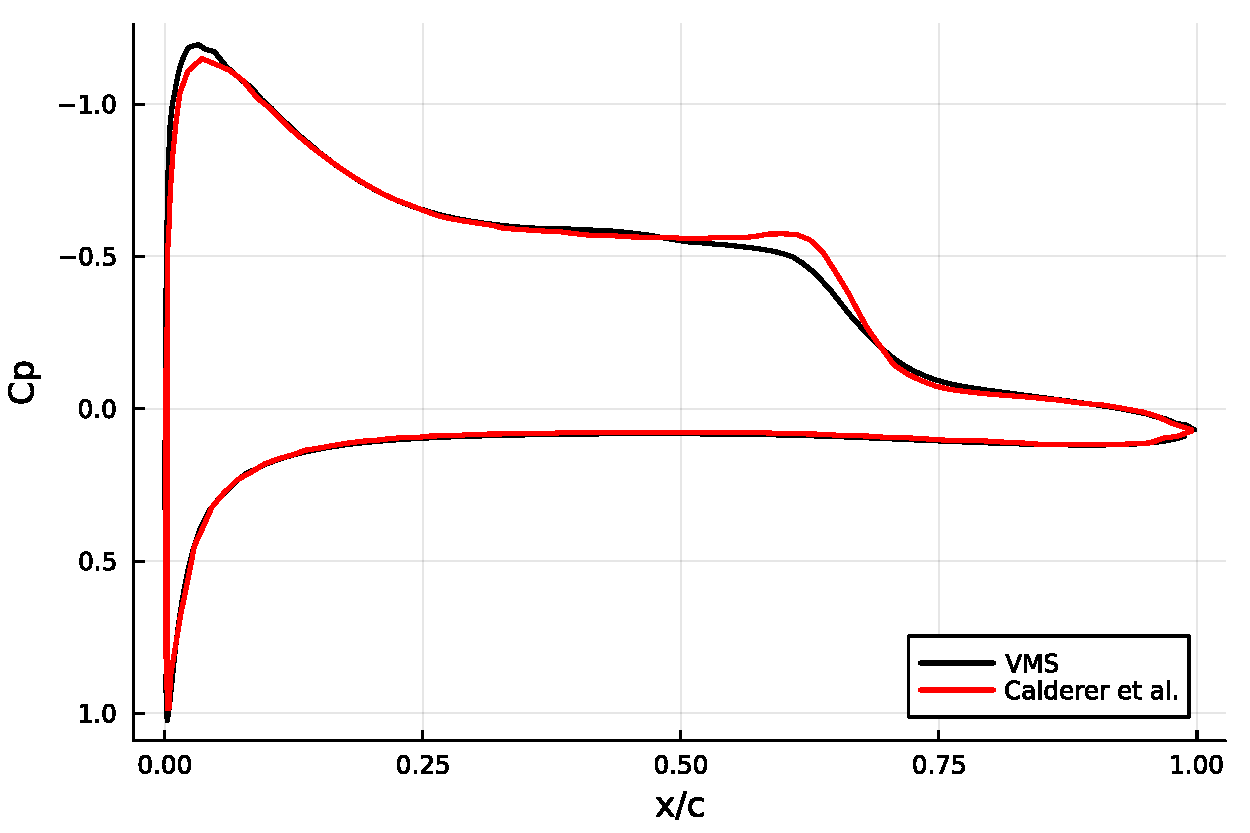
\includegraphics[width=\textwidth]{sd7003_cp.pdf}
     \end{subfigure}
\caption{Comparison with VMS literature results}
     \end{figure} 
     
\end{frame}

\begin{frame}{ VMS linearized coupled sd7003s}
\begin{figure}[h]
     \centering          
         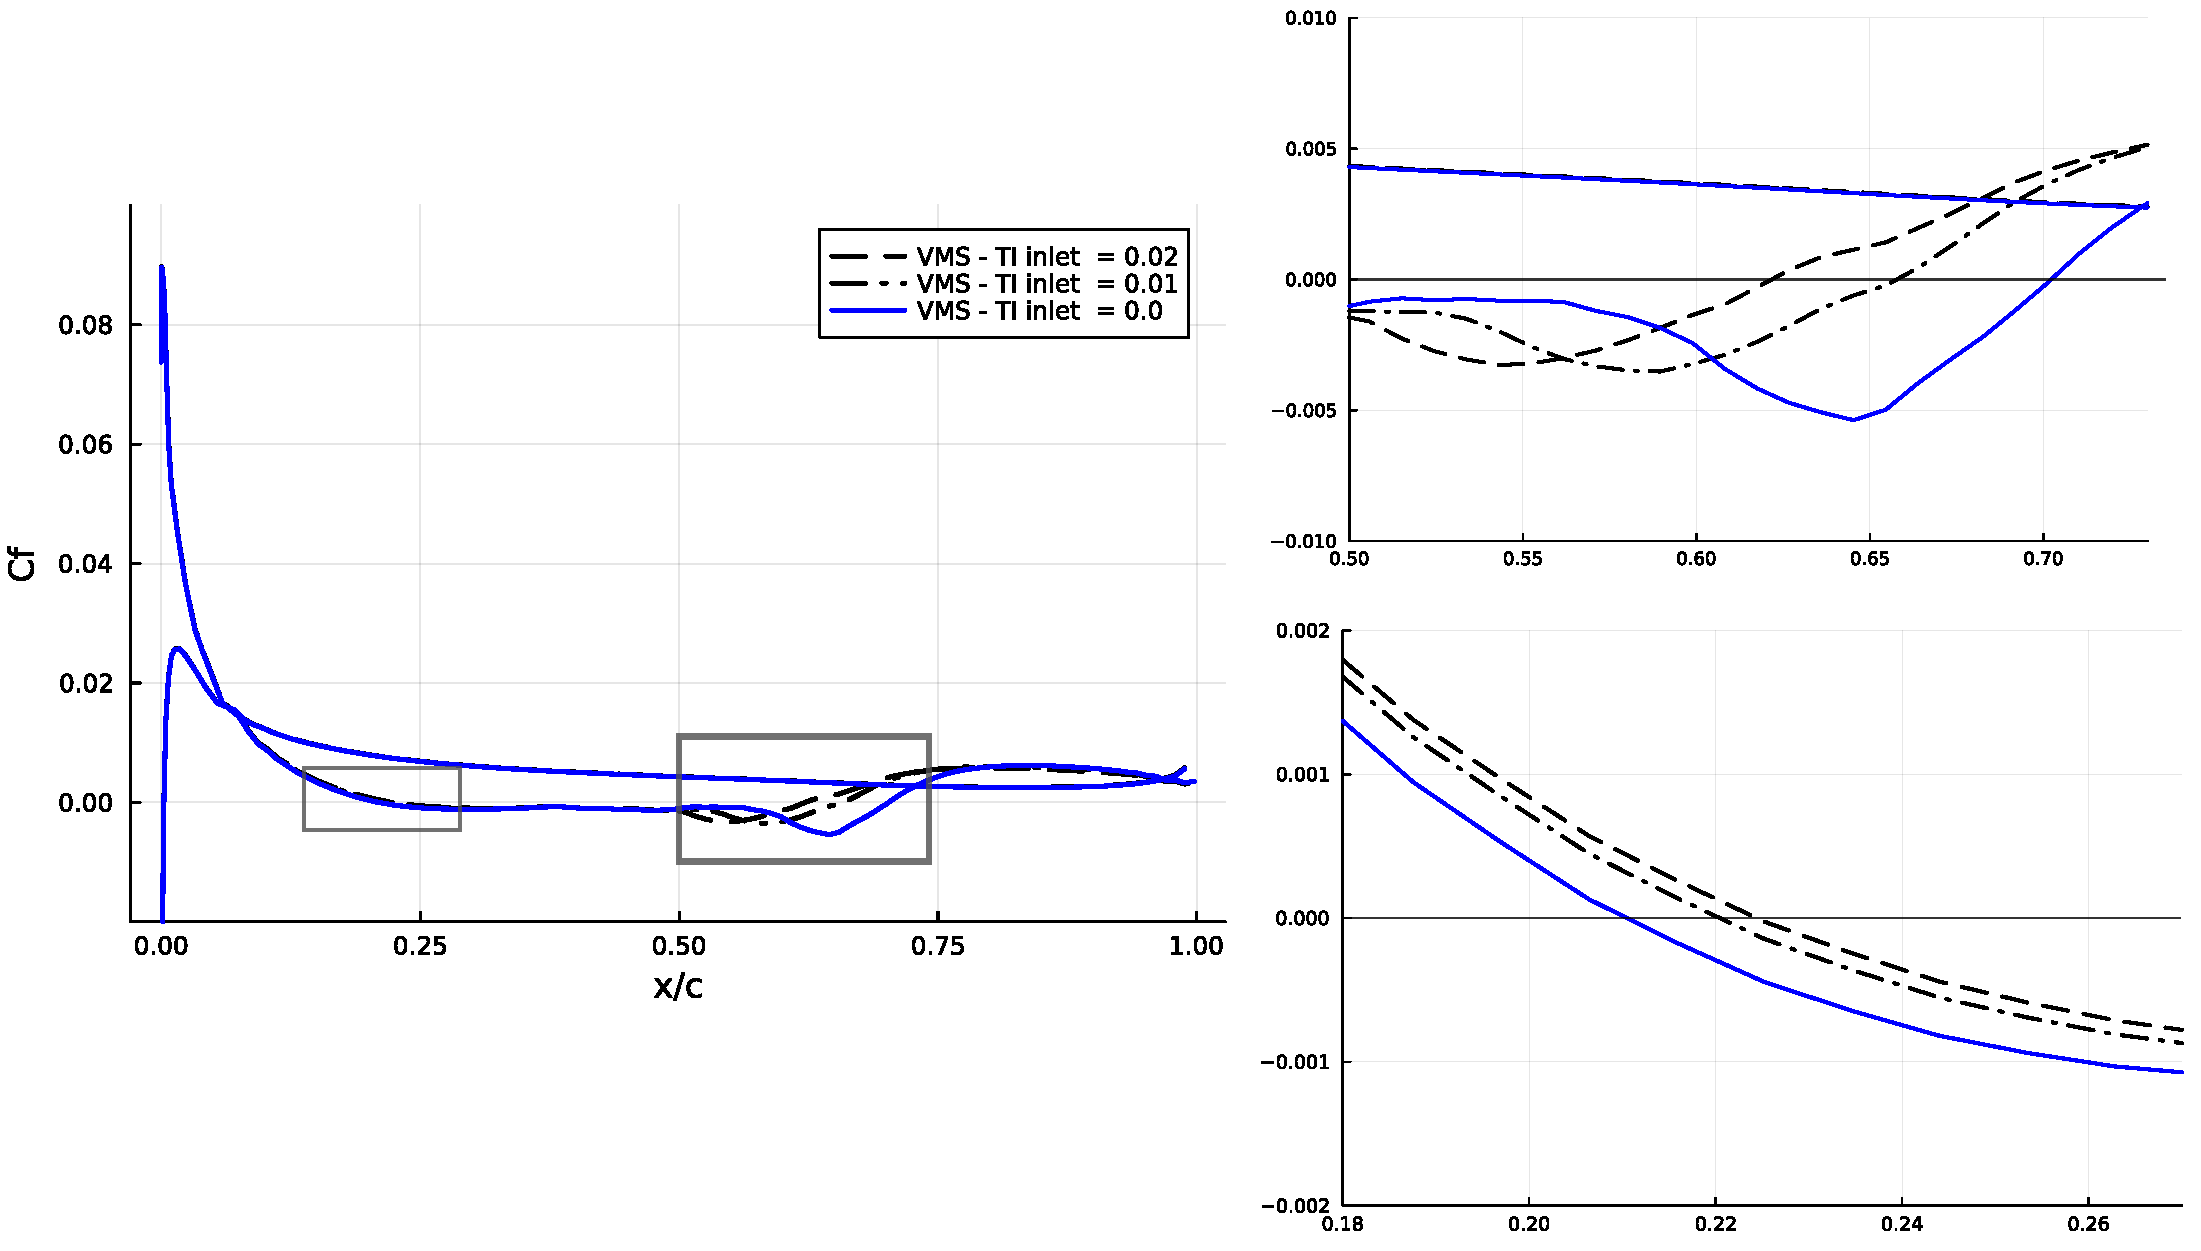
\includegraphics[width=0.8\textwidth]{SD7003_Cf_zoom.pdf}
         \caption{Bubble position function of freestream turbulence intensity}
     \end{figure} 
\end{frame}




\begin{frame}{VMS Linearized-Segregated}
Segregated: each time step pressure and velocity system are solved one after the other multiple times. It is possible to re-use the matrices and preconditioner. It is an iterative method.

\end{frame}




\begin{frame}{VMS Linearized-Segregated}
PhD research aims to simulate new a new airfoil.
Re $\num{250000}$ - AoA $\ang{1}$ 

\begin{figure}[h]
     \centering          
     \begin{subfigure}[h]{0.45\textwidth}
              \centering
         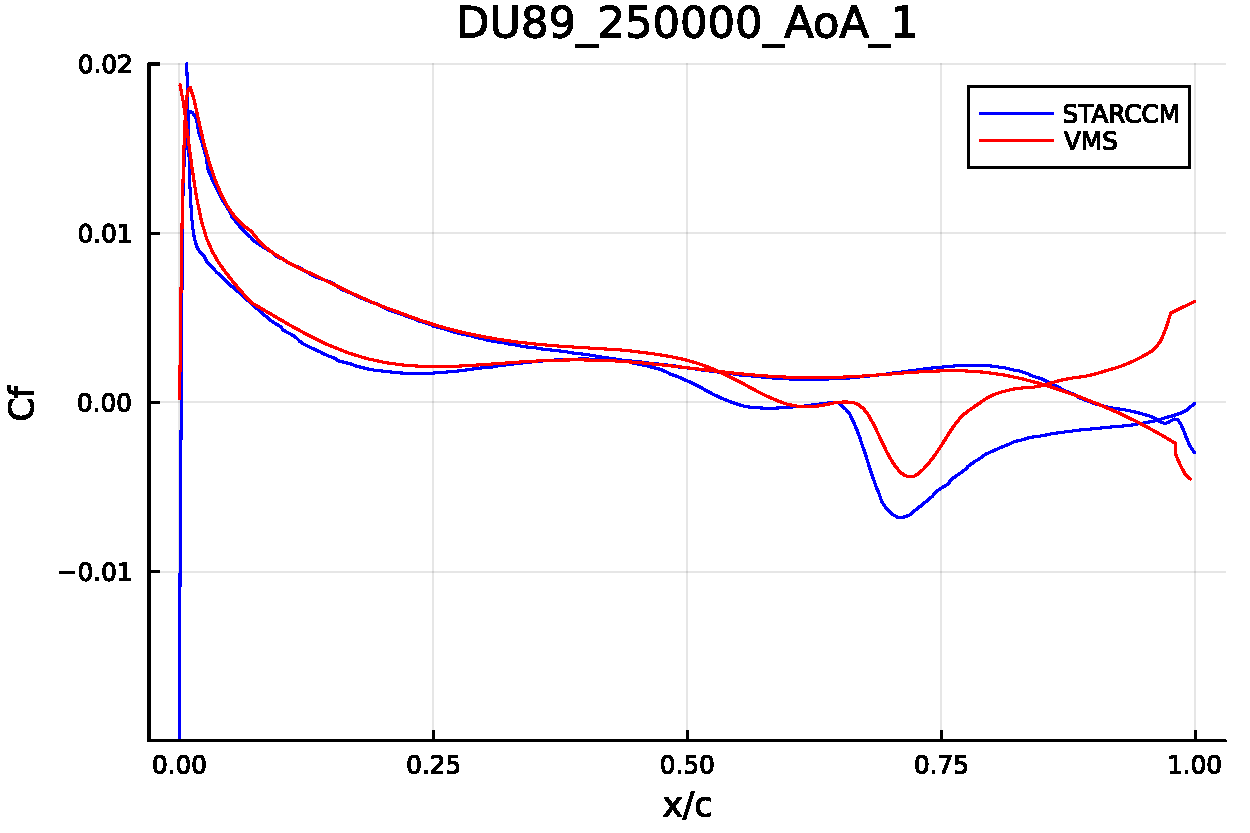
\includegraphics[width=\textwidth]{DU89_250000_AoA_1_Cf.pdf}
    \end{subfigure}
          \hfill
     \begin{subfigure}[h]{0.45\textwidth}
      \centering
         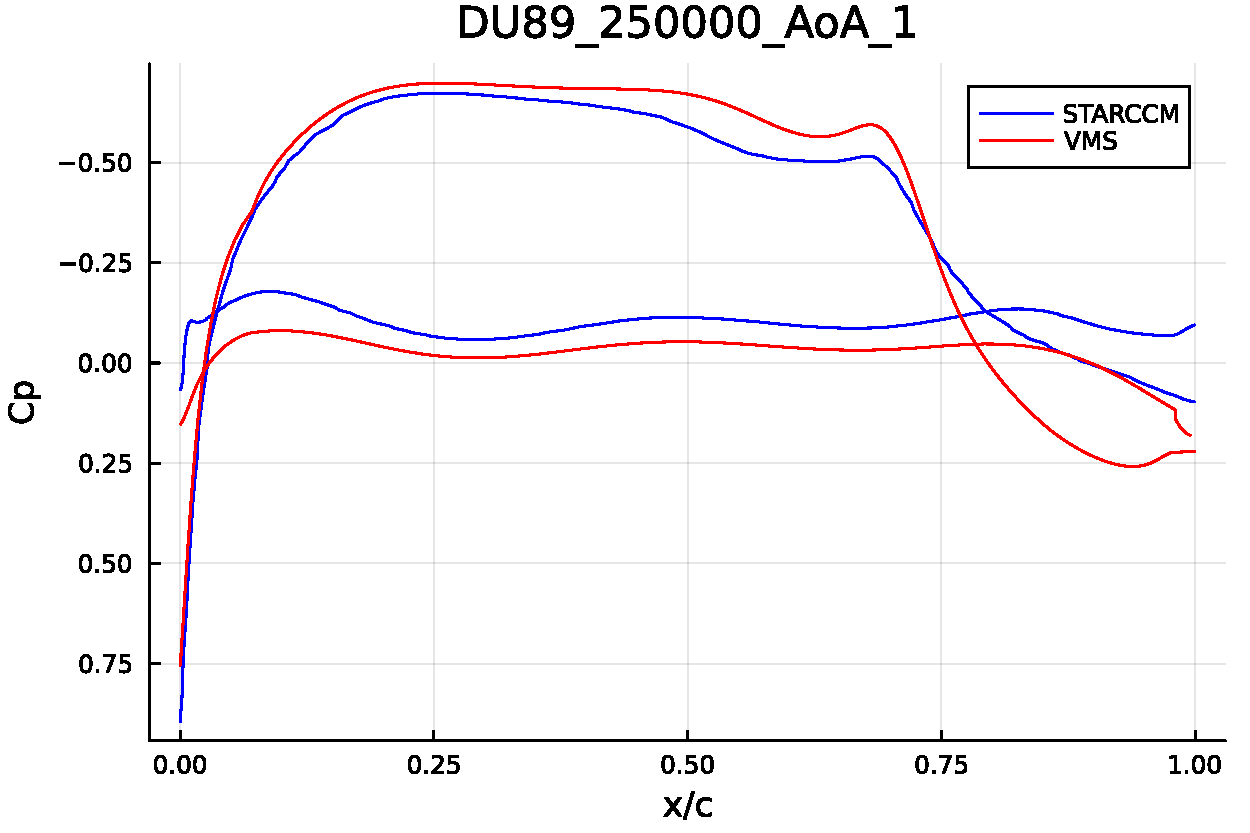
\includegraphics[width=\textwidth]{DU89_250000_AoA_1_Cp.pdf}
     \end{subfigure}
     \end{figure} 
 \end{frame}

\begin{frame}{VMS Linearized-Segregated}
Re $\num{250000}$ - AoA $\ang{5}$ 
\begin{figure}[h]
     \centering          
     \begin{subfigure}[h]{0.45\textwidth}
              \centering
         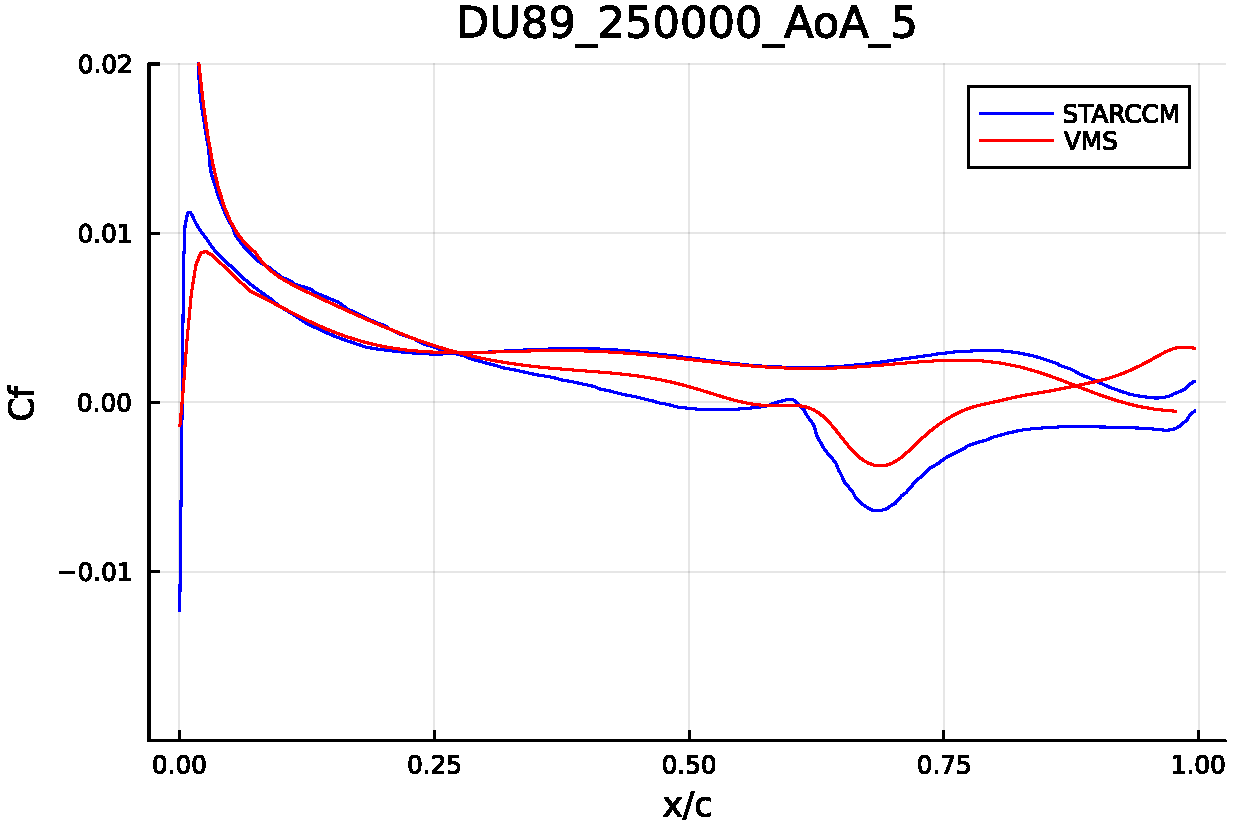
\includegraphics[width=\textwidth]{DU89_250000_AoA_5_Cf.pdf}
    \end{subfigure}
          \hfill
     \begin{subfigure}[h]{0.45\textwidth}
      \centering
         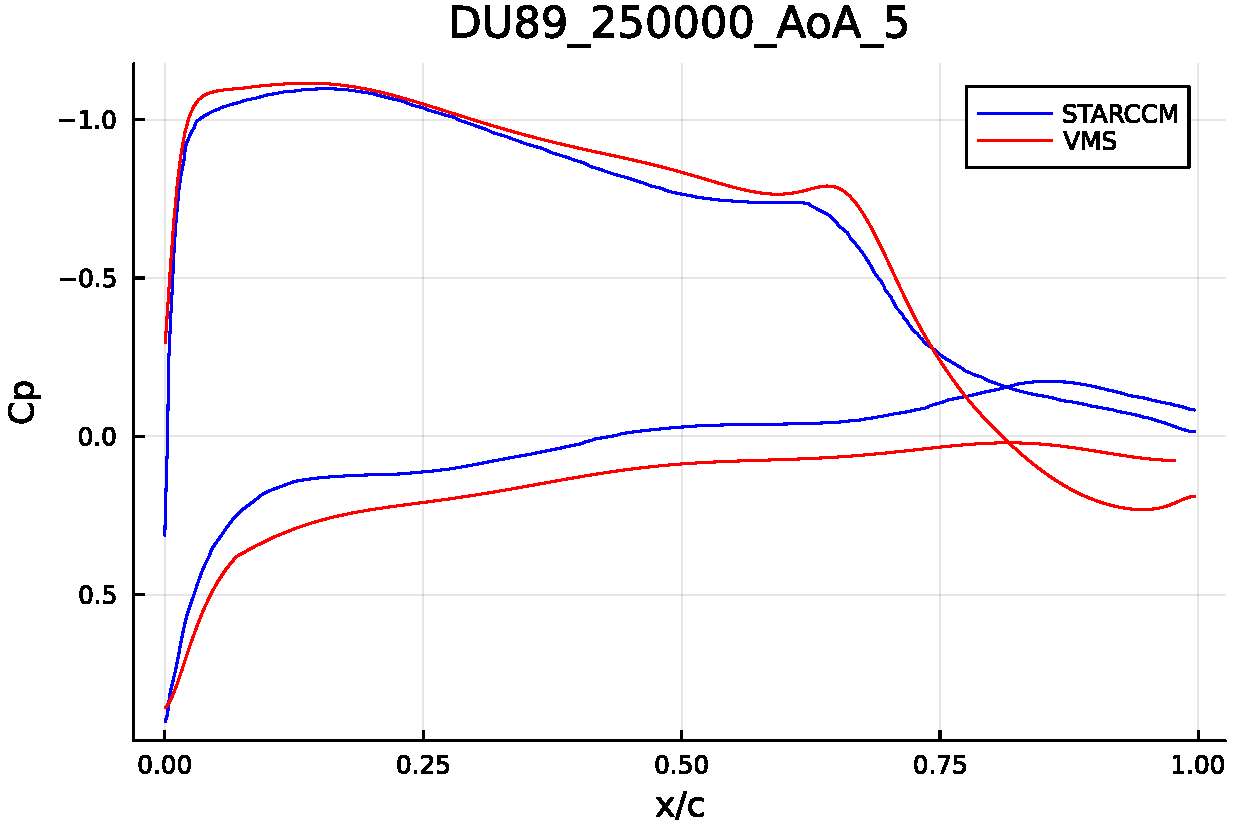
\includegraphics[width=\textwidth]{DU89_250000_AoA_5_Cp.pdf}
     \end{subfigure}
     \end{figure} 
 \end{frame}

\begin{frame}{VMS Linearized-Segregated}
Re $\num{500000}$ - AoA $\ang{1}$ 
\begin{figure}[h]
     \centering          
     \begin{subfigure}[h]{0.45\textwidth}
              \centering
         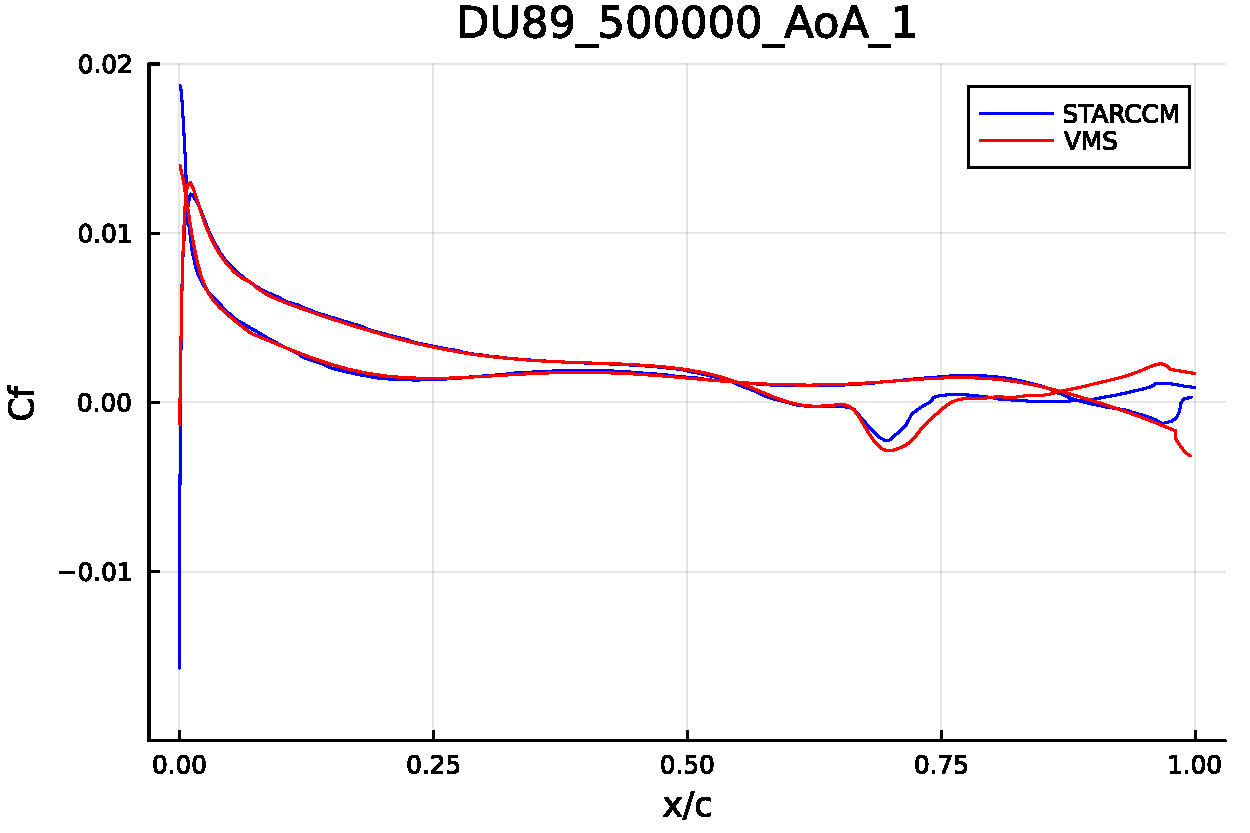
\includegraphics[width=\textwidth]{DU89_500000_AoA_1_Cf.pdf}
    \end{subfigure}
          \hfill
     \begin{subfigure}[h]{0.45\textwidth}
      \centering
         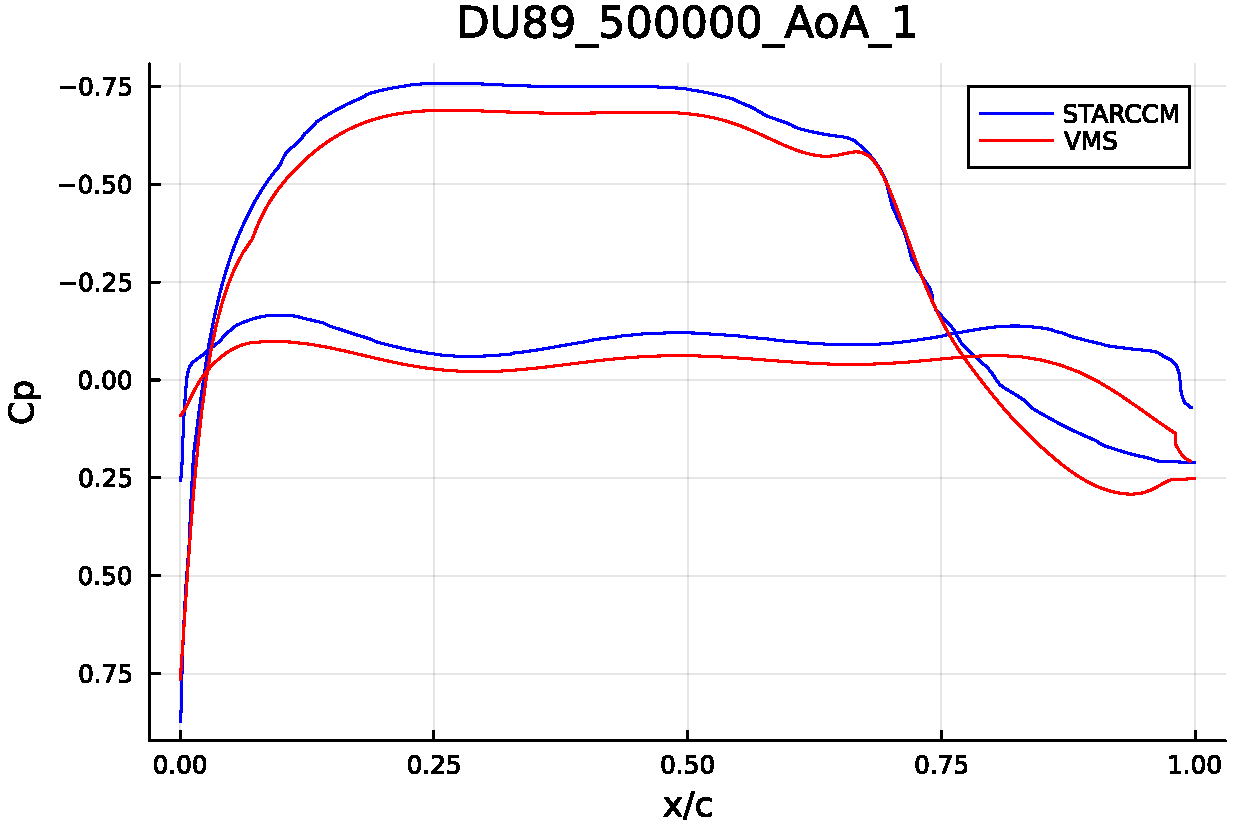
\includegraphics[width=\textwidth]{DU89_500000_AoA_1_Cp.pdf}
     \end{subfigure}
     \end{figure} 
 \end{frame}

\begin{frame}{VMS Linearized-Segregated}
Re $\num{500000}$ - AoA $\ang{5}$ 
\begin{figure}[h]
     \centering          
     \begin{subfigure}[h]{0.45\textwidth}
              \centering
         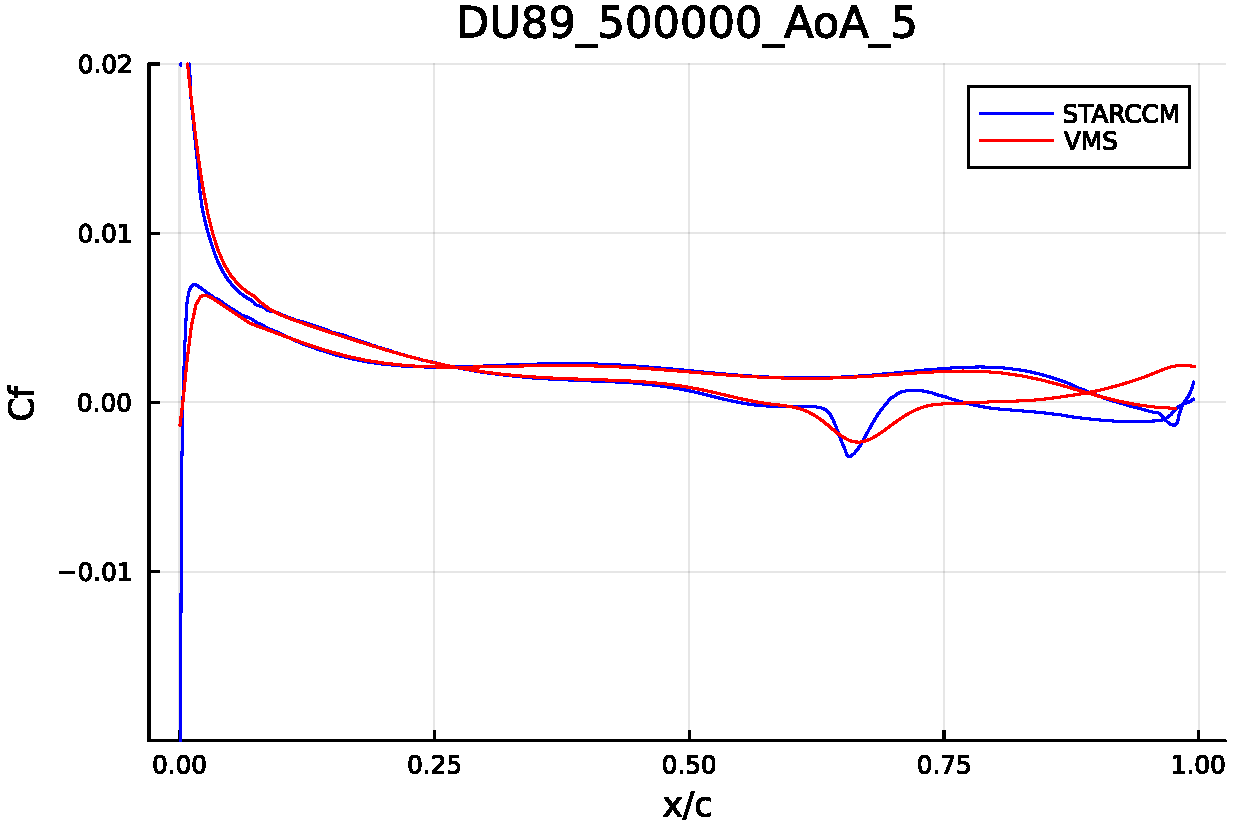
\includegraphics[width=\textwidth]{DU89_500000_AoA_5_Cf.pdf}
    \end{subfigure}
          \hfill
     \begin{subfigure}[h]{0.45\textwidth}
      \centering
         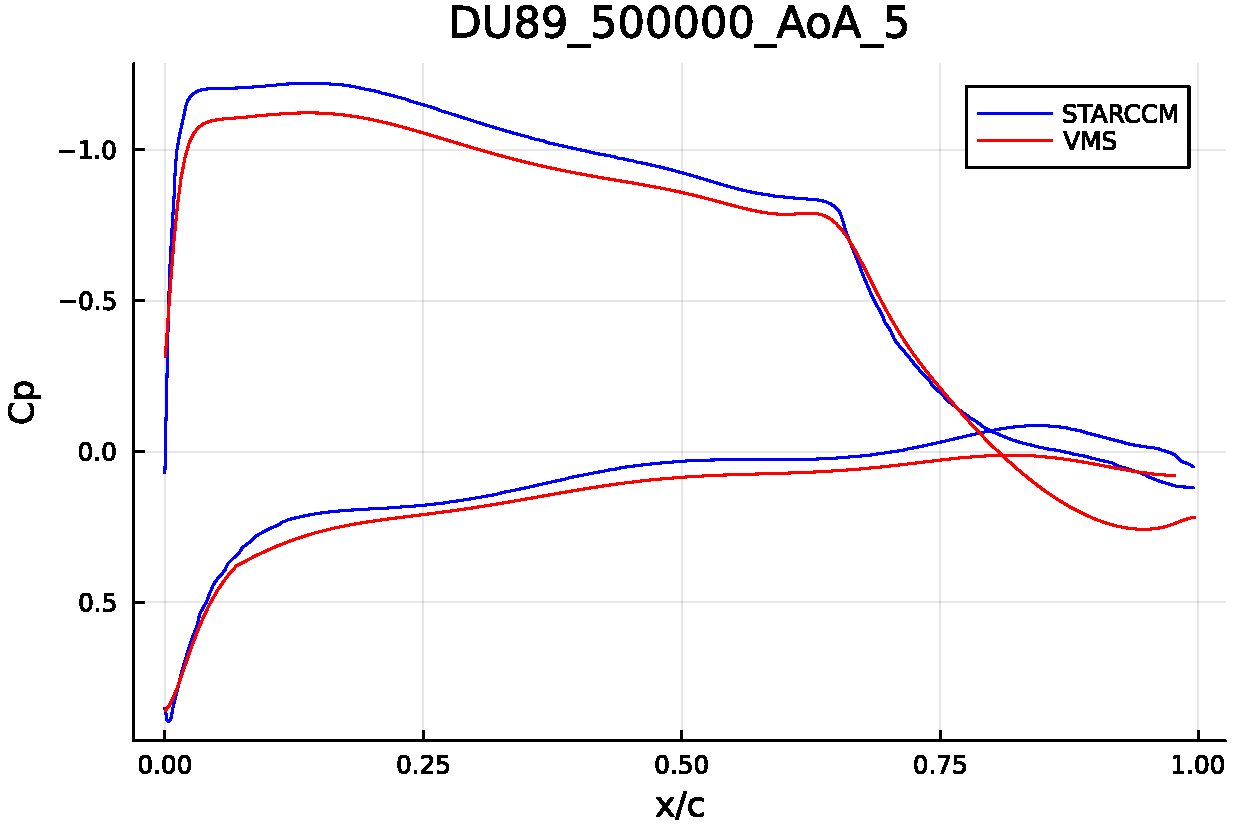
\includegraphics[width=\textwidth]{DU89_500000_AoA_5_Cp.pdf}
     \end{subfigure}
     \end{figure} 
 \end{frame}





\section{Other activities}
\begin{frame}{Other activities}
\begin{itemize}
	\item Synthetic Eddy Method \href{https://www.theoj.org/joss-papers/joss.05565/10.21105.joss.05565.pdf}{publication}
	\item JuliaCon 2023 conference
	\item Co-author AIAA 2023 conference paper
\end{itemize}

\begin{itemize}
	\item Testing standard passive flow controls (no improvment in aerodynamic efficiency)
\end{itemize}

\end{frame}



\section{Element of novelty}
\begin{frame}{Elements of novelty}
\begin{itemize}
	\item Systematic usage of Julia in fluid-dynamics
	\item Usage of VMS for high Reynolds airfoil
	\item First LES code in Julia - fully parallelized - working with 3D airfoils up to Re $\num{500000}$ 
	\item Synthetic Eddy Method coded in Julia and coupled with the VMS
\end{itemize}

It has been challenging, but it seems we are on the right path!

\end{frame}

\section{Next steps}
\begin{frame}{Next steps}
Expected papers:
\begin{itemize}
	\item VMS paper (prof. Janssens reading)
	\item Experimental validation of the LS-VMS - publish paper
	\item LC-VMS - (publish paper?)
\end{itemize}

Expected conferences:
\begin{itemize}
	\item AIAA2024 conferences (LS-VMS, LC-VMS)
	\item DLES14 (VMS usage, validation test cases)
	\item ICAS2024 (Passive Flow Controls)
\end{itemize}


Expected research:
\begin{itemize}
	\item Uncertainty Quantification using Polynomials Chaos Transformation
	\item Start coding the adjoint optimization
	\item Test a passive flow control with the VMS
\end{itemize}

\end{frame}



\end{document}
